% Adapted from the distributed IEEEtran bare_jrnl.tex, V1.4b, Michael Shell.
% TMM figure replacement, independent copy dated 2026-10-20.
\ifdefined\pdfminorversion\pdfminorversion=7\fi
\documentclass[10pt,journal,letterpaper]{IEEEtran}
% SPS manuscript guidelines specify double-column 10pt and one-inch margins.
\usepackage[margin=1in]{geometry}
\usepackage{cite}
\usepackage{graphicx}
\usepackage{amsmath,amssymb,amsfonts,mathtools}
\usepackage{booktabs,multirow,array}
\usepackage{xspace}
\usepackage{microtype}
\usepackage{needspace}
\usepackage{placeins}
\raggedbottom
\usepackage[hidelinks]{hyperref}
\newcommand{\ours}{DEDBSR\xspace}
\newcommand{\lr}{\mathrm{LR}}
\newcommand{\hr}{\mathrm{HR}}
\newcommand{\teacher}{\mathrm{T}}
\newcommand{\student}{\mathrm{S}}
\newcommand{\best}[1]{\textbf{#1}}
\newcommand{\second}[1]{\underline{#1}}
\hyphenation{super-resolution re-con-struc-tion}
\hyphenation{trans-form deg-ra-da-tion con-trast-ive spa-tial}

% Compact float placement; preserve IEEEtran typography and page geometry.
\setcounter{topnumber}{4}
\setcounter{dbltopnumber}{4}
\setcounter{totalnumber}{6}
\renewcommand{\topfraction}{0.95}
\renewcommand{\dbltopfraction}{0.95}
\renewcommand{\textfraction}{0.05}
\renewcommand{\floatpagefraction}{0.8}
\renewcommand{\dblfloatpagefraction}{0.8}
\setlength{\textfloatsep}{12pt plus 2pt minus 2pt}
\setlength{\dbltextfloatsep}{12pt plus 2pt minus 2pt}
\setlength{\floatsep}{10pt plus 2pt minus 2pt}
\setlength{\dblfloatsep}{10pt plus 2pt minus 2pt}
\makeatletter
\setlength{\@fptop}{0pt}
\setlength{\@fpsep}{10pt plus 1pt minus 1pt}
\setlength{\@fpbot}{0pt plus 1fil}
\setlength{\@dblfptop}{0pt}
\setlength{\@dblfpsep}{10pt plus 1pt minus 1pt}
\setlength{\@dblfpbot}{0pt plus 1fil}
\makeatother

\title{DEDBSR: Deep Ensemble Distillation for Blind Image Super-Resolution}
% Author names/order/affiliations were not supplied in the source draft.
% Fill with verified author information before submission.
\author{}

\markboth{DEDBSR: Manuscript for IEEE Transactions on Multimedia}{DEDBSR}
\begin{document}
\maketitle

\begin{abstract}
Blind image super-resolution (BSR) reconstructs a high-resolution image from a low-resolution observation with unknown blur and noise. Recent distillation-based BSR methods transfer degradation representations to LR-only models, while how this guidance should evolve across restoration depth remains insufficiently explored. Our Fourier analysis of reconstructions at different execution depths shows depth-dependent restoration errors, motivating guidance that accounts for deeper computation and interactions between stages. We propose DEDBSR, a deep ensemble distillation framework that propagates channel and spatial conditions through recurrent restoration groups, forms a degradation-guided ensemble of their residual corrections, and transfers this depth-aware restoration path to an LR-only branch. The LR-only branch inherits the privileged restoration generator and adapts through condition distillation and GT-guided supervision, which combines ground-truth reconstruction with output imitation selected by relative reconstruction error. Experiments on standard blind-SR and anisotropic/noisy benchmarks demonstrate competitive performance under diverse degradations.

\end{abstract}
\begin{IEEEkeywords}
Blind image super-resolution, knowledge distillation, degradation conditioning, residual ensemble.
\end{IEEEkeywords}

\begin{figure*}[t]
\centering
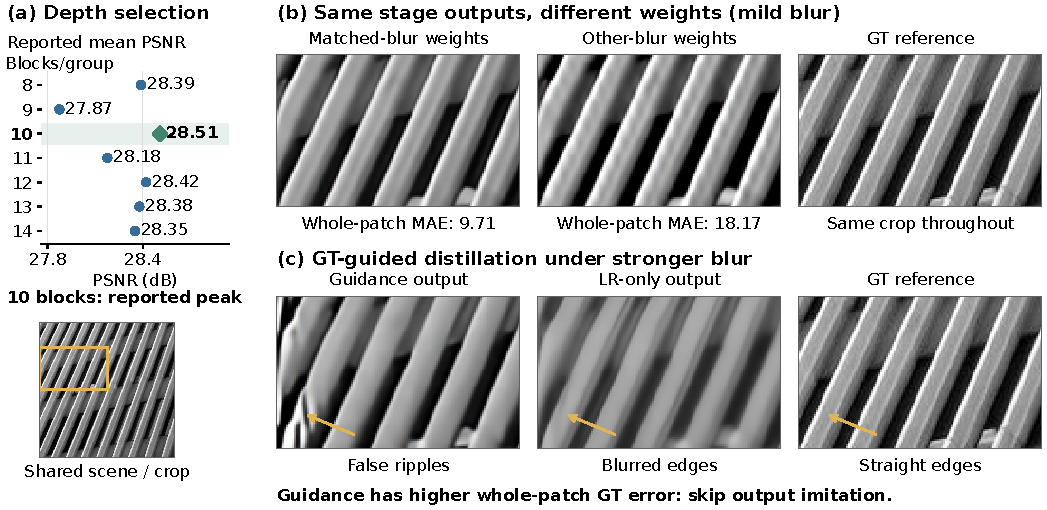
\includegraphics[width=\textwidth]{figures/motivation/motivation_visual_v39.pdf}
\caption{\textbf{Depth selection, stage composition, and GT-guided distillation.} (a) Ten blocks give the highest reported mean; retest limitations are in the supplement. (b,c) The same boxed scene region under different blur conditions. (b) Using the combination predicted for another blur condition increases error while keeping the input and stage corrections fixed. MAE is measured over the full patch on the 0--255 RGB scale. (c) Degradation-informed guidance contains false ripples and has higher whole-patch GT error than the blurrier LR-only output: skip output imitation, retain GT reconstruction. Selection uses whole-patch errors, not crop errors or pixelwise masks. This selected example does not establish a training gain.}
\label{fig:motivation}
\end{figure*}

\section{Introduction}
\label{sec:intro}

Blind image super-resolution (BSR) reconstructs a high-resolution (HR) image from a low-resolution (LR) observation when the blur, downsampling, and noise that produced the observation are unknown. The degradation removes high-frequency structures and makes the desired inverse mapping input-dependent: a model must infer which details are supported by the observation before it restores them. Existing BSR systems therefore couple reconstruction with degradation estimation or representation learning, but the guidance still has to remain useful as the reconstruction proceeds through a deep generator.

Existing BSR methods estimate explicit degradation parameters or learn implicit representations to condition reconstruction. Iterative kernel correction and alternating estimation--restoration exemplify the former, while contrastive degradation learning exemplifies the latter~\cite{gu2019ikc,luo2020dan,wang2021dasr}. More recently, knowledge distillation has enabled training-only information to support LR-only inference. KDSR and LightBSR, for example, transfer degradation-aware representations learned with LR--HR pairs~\cite{xia2023kdsr,yuan2025lightbsr}. Building on this setting, we study how transferred conditions are propagated across restoration stages, how stage corrections are combined, and when output guidance should be imitated.

These considerations link restoration depth, stage interaction, and guidance reliability. First, useful computation across depth should be preserved during transfer. Our Fourier analysis shows that executing more blocks of the same trained network can reduce mean frequency-domain reconstruction errors (Sec.~\ref{sec:depth}). The separate architectural sweep in Fig.~\ref{fig:motivation}(a) gives the highest reported mean at ten blocks per group, providing our reference depth. Second, depth-dependent restoration motivates examining how degradation conditions evolve between groups and how their corrections are combined. Figure~\ref{fig:motivation}(b) isolates the composition aspect: under mild blur, using a stage combination predicted for another blur condition increases error while keeping the input and all group corrections fixed. Third, privileged output guidance can be less accurate than the LR-only prediction. For the same scene under stronger blur, Fig.~\ref{fig:motivation}(c) shows false ripples in the privileged output, whereas the blurrier LR-only output has lower whole-patch error against ground truth (GT). This motivates GT-based output selection while retaining GT reconstruction for every patch.

We propose DEDBSR, a deep ensemble distillation framework that transfers a degradation-informed restoration path to LR-only inference. A kernel-informed privileged branch learns the restoration computation; the LR-only branch inherits and adapts it through condition distillation and GT-guided supervision. The framework integrates recurrent condition propagation, stage-wise residual aggregation, and selective output imitation. Our main contributions are summarized as follows:

\begin{itemize}
\item We propose a deep ensemble distillation framework for blind SR that transfers a trained restoration path to an LR-only model. GT-guided supervision combines reconstruction with output imitation selected according to relative reconstruction error.
\item We develop two modules for cross-stage restoration: degradation recurrent groups propagate channel and spatial conditions, while a degradation-guided residual ensemble combines completed group corrections. Together, they connect condition evolution with stage composition.
\item Experiments demonstrate competitive performance on standard BSR benchmarks under isotropic and anisotropic/noisy degradations. Further analyses examine the roles of restoration depth, stage interaction, and GT-guided supervision.
\end{itemize}

\section{Related Work}
\label{sec:related_work}

\noindent\textbf{Degradation modeling for blind SR.}
Blind SR handles unknown degradations through internal learning, explicit estimation, or implicit representations. ZSSR adapts to a test image, while KernelGAN estimates its kernel from internal statistics~\cite{shocher2018zssr,bellkligler2019kernelgan}; learned kernel priors and probabilistic noise modeling further constrain estimation~\cite{liang2021fkp,yue2022bsrdm}. Unlike SRMD and USRNet, which use supplied degradation information~\cite{zhang2018srmd,zhang2020usrnet}, IKC, DAN, and DCLS couple estimation with reconstruction~\cite{gu2019ikc,luo2020dan,luo2022dcls}. Implicit methods instead learn conditions through contrastive or meta-learning objectives~\cite{wang2021dasr,xia2023mrda}, incorporate them into attention or predict joint content--degradation priors~\cite{liu2024dsat,liu2024cdformer}, and reduce content interference~\cite{chen2025drat,yuan2025cdcl}. Separately, BSRGAN and Real-ESRGAN broaden synthetic training degradations~\cite{zhang2021bsrgan,wang2021realesrgan}. These directions address different parts of the blind inverse problem: estimating the imaging process, learning a useful restoration condition, and covering the degradations encountered at test time. An informative condition must also be integrated into the reconstruction network; its representation alone does not determine how successive stages should use it.

\noindent\textbf{Deep and conditional restoration.}
Recursion, dense feature reuse, and residual channel attention support deep SR~\cite{tai2017drrn,zhang2018rdn,zhang2018rcan}; back-projection and second-order attention provide feedback and feature-correlation modeling~\cite{haris2018dbpn,dai2019san}. SwinIR, HAT, and SRFormer expand spatial interactions through shifted, overlapping, or permuted attention~\cite{liang2021swinir,chen2023hat,zhou2023srformer}. Token dictionaries and state-space models further extend context aggregation~\cite{zhang2024atd,guo2024mambair,guo2025mambairv2}, while high-pass filtering and frequency-aware attention target detail recovery~\cite{magid2021dynamic,dai2024freqformer}. Conditioning is also established: SFT applies semantic spatial modulation~\cite{wang2018sft}, and conditional or dynamic convolutions adapt operators to input signals~\cite{yang2019condconv,chen2020dynamicconv,xu2020udvd}. These mechanisms distinguish feature interaction and conditional computation from merely increasing depth. RDN and RCAN establish hierarchical reuse and deep residual processing, whereas attention and state-space approaches primarily expand the spatial information available to a feature. SFT uses semantic priors, while UDVD assumes supplied degradation information. This distinction separates the source of guidance from the location where it modifies computation, and separates feature transformation from aggregation of completed stage corrections.

\noindent\textbf{Restoration distillation.}
SR distillation uses HR-privileged information~\cite{lee2020pisr}, feature affinities~\cite{he2020fakd}, or synthesized inputs when training data are unavailable~\cite{zhang2021dfkd}. MTKD combines multiple predictions with wavelet supervision~\cite{jiang2024mtkd}; MiPKD mixes feature- and block-level priors~\cite{li2025mipkd}; DCKD adjusts contrastive guidance to the student's learning state~\cite{zhou2025dckd}. For blind SR, KDSR and LightBSR transfer degradation representations to LR-only models~\cite{xia2023kdsr,yuan2025lightbsr}. Existing work therefore already addresses intermediate knowledge and adaptive supervision. In particular, feature-affinity and prior-mixing approaches show that distillation need not be restricted to final predictions; multi-teacher and adaptive contrastive approaches also modify the guidance supplied during learning. KDSR and LightBSR provide the closest blind-SR setting because training-only information must become useful to a branch that observes LR alone. The remaining design questions concern how transferred guidance enters successive restoration stages and how imitation targets relate to reconstruction accuracy.

\noindent\textbf{Generative restoration priors.}
StableSR, DiffBIR, and SeeSR adapt pretrained diffusion priors through restoration or semantic conditioning~\cite{wang2024stablesr,lin2024diffbir,wu2024seesr}. ResShift redesigns the sampling process~\cite{yue2023resshift}, while SinSR, OSEDiff, and TSD-SR pursue single-step restoration through distinct distillation objectives~\cite{wang2024sinsr,wu2024osediff,dong2025tsdsr}. These approaches emphasize generative detail and sampling efficiency rather than condition propagation within a feed-forward restoration path. Their restoration objectives and real-world degradation protocols also differ from controlled Gaussian comparisons, so perceptual synthesis and distortion-oriented reconstruction require separate evidence.


\section{Proposed Method}
\label{sec:method}

\subsection{Overview and Notation}
\label{sec:overview}

\looseness=-1
Figure~\ref{fig:architecture} separates the restoration path from the training-only supervision paths. Let $\mathbf y\in\mathbb R^{3\times H\times W}$ be an LR image and $\mathbf x\in\mathbb R^{3\times rH\times rW}$ its HR target, related by $\mathbf y=(\mathbf x*\mathbf k)\!\downarrow_r+\mathbf n$. Here $\mathbf k$ is a blur kernel, $r$ is the scale factor, and $\mathbf n$ is additive noise. The privileged branch, denoted by $P$, receives $\mathbf y$ and a spatially broadcast PCA encoding $\mathbf d(\mathbf k)$ of the kernel. The LR-only branch, denoted by $L$, receives only $\mathbf y$.

\looseness=-1
Each branch has a condition encoder, a convolutional stem, a stack of degradation recurrent groups (DRGs), degradation-guided dynamic weighting (DG), and a reconstruction head. Both generators have the same architecture, but their parameters are separate after initialization. We use $a\in\{P,L\}$ to index branches and omit this superscript on learnable operators when the branch is clear. The condition states are $\mathbf c_i^a\in\mathbb R^{d_c}$ and $\mathbf s_i^a\in\mathbb R^{d_s\times H\times W}$; the restoration features are $\mathbf f_i^a\in\mathbb R^{C\times H\times W}$. There are $N$ groups and $M$ degradation-modulated blocks (DMBs) per group. We write $[\cdot,\cdot]$ for channel concatenation, $\odot$ for elementwise multiplication with broadcasting, $\phi$ for GELU, and $\sigma$ for the sigmoid function. The framework's encoder lanes, panels (a)--(d), and three-input GT supervision path correspond to the components below.

\begin{figure*}[!t]
\centering
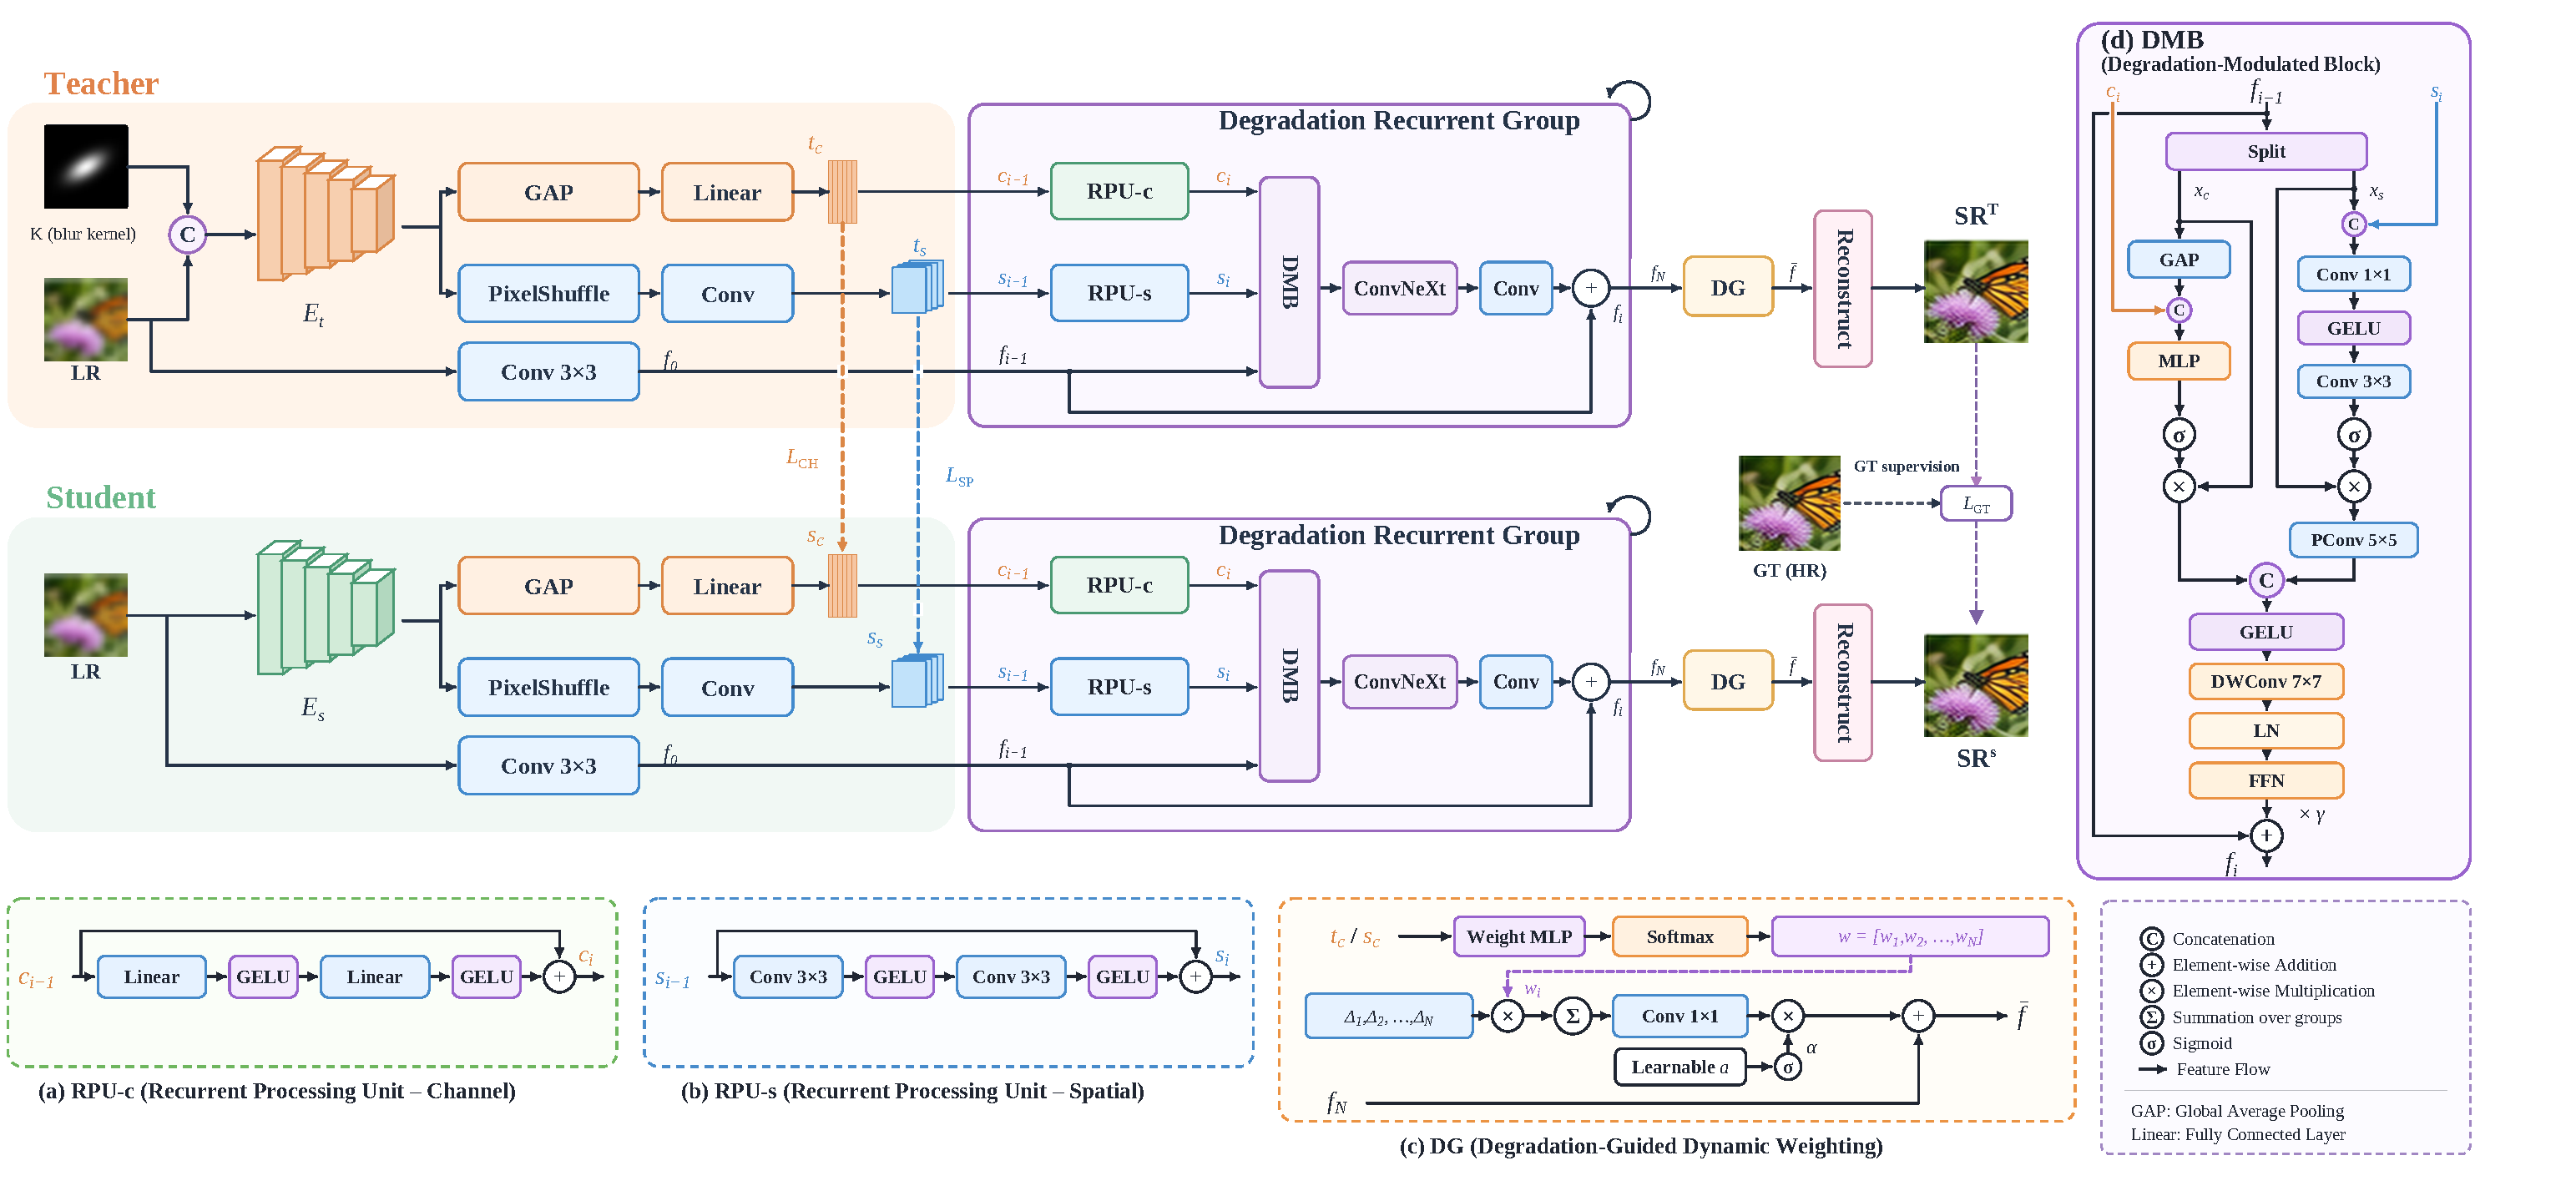
\includegraphics[width=\textwidth]{figures/distillation_framework_three_inputs_v32_checked_vector.pdf}
\caption{\textbf{DEDBSR restoration and distillation framework.} The privileged branch receives an LR image and a kernel-derived condition map, while the LR-only branch receives the LR image alone. The encoder heads supply initial channel and spatial conditions. RPU-c and RPU-s, expanded in (a,b), update the conditions before each degradation recurrent group. DMB in (d) applies channel and spatial modulation; DG in (c) weights completed group corrections. Reconstruct includes the output projection, global stem skip, and upsampling head. Dashed condition paths align the initial conditions. The three-input GT supervision block uses both reconstructions and GT to combine GT reconstruction with selective output imitation. The LR-only generator inherits the privileged generator at initialization; only the LR-only branch is used at inference.}
\label{fig:architecture}
\end{figure*}

\begingroup
\predisplaypenalty=0
\subsection{Condition Encoding}
\label{sec:condition_encoding}

The condition encoders extract guidance separately from the features used for reconstruction. In the two encoder lanes of Fig.~\ref{fig:architecture},
\begin{equation}
\mathbf q^P=E_P([\mathbf y,\mathbf d(\mathbf k)]),\qquad
\mathbf q^L=E_L(\mathbf y).
\label{eq:encoder}
\end{equation}
\endgroup
The privileged encoder recalibrates convolutional features through squeeze-and-excitation. The LR-only encoder has a separate convolutional path. The two encoders produce condition features with compatible shapes and use separate parameters.

The GAP--Linear and PixelShuffle--Conv heads convert the encoder features in Eq.~\eqref{eq:encoder} into the initial conditions:
\begin{equation}
\begin{aligned}
\mathbf c_0^a&=\phi\!\left(A_c^a(\operatorname{GAP}(\mathbf q^a))\right),\\
\mathbf s_0^a&=\phi\!\left(K_s^a(\mathcal A(\operatorname{PS}(\mathbf q^a)))\right).
\end{aligned}
\label{eq:initcond}
\end{equation}
Here $A_c^a$ is a learned linear projection, $K_s^a$ is a convolution, $\operatorname{PS}$ denotes pixel shuffle, and $\mathcal A$ aligns the condition map to the LR grid when boundary padding is required. The initial channel condition supports channel modulation and DG weight prediction; the spatial condition supports spatial modulation. A separate stem produces $\mathbf f_0^a=F_a(\mathbf y-\boldsymbol\mu)$, where $\boldsymbol\mu$ is the RGB mean removed by the generator. The pairs $(t_c,t_s)$ and $(s_c,s_s)$ in the figure denote $(\mathbf c_0^P,\mathbf s_0^P)$ and $(\mathbf c_0^L,\mathbf s_0^L)$, respectively. They are connected by the channel and spatial distillation paths.

\subsection{Degradation Recurrent Groups}
\label{sec:drg}

The DRG stack propagates condition states together with the restoration features. Starting from Eq.~\eqref{eq:initcond}, the channel and spatial recurrent processing units, RPU-c and RPU-s in Fig.~\ref{fig:architecture}(a,b), update the states before group $i$:
\begin{equation}
\begin{aligned}
\mathbf c_i^a&=\mathbf c_{i-1}^a+U_{c,i}(\mathbf c_{i-1}^a),\\
\mathbf s_i^a&=\mathbf s_{i-1}^a+U_{s,i}(\mathbf s_{i-1}^a).
\end{aligned}
\label{eq:update}
\end{equation}
The implementation uses a residual channel MLP and a residual spatial convolutional mapping:
\begin{equation}
\begin{aligned}
U_{c,i}(\mathbf c)&=\phi\!\left(A_{c,i}^{(2)}(\phi(A_{c,i}^{(1)}(\mathbf c)))\right),\\
U_{s,i}(\mathbf s)&=\phi\!\left(K_{s,i}^{(2)}(\phi(K_{s,i}^{(1)}(\mathbf s)))\right).
\end{aligned}
\label{eq:rpu_maps}
\end{equation}
The affine maps $A_{c,i}^{(\cdot)}$ and convolutions $K_{s,i}^{(\cdot)}$ preserve the output dimensions of the corresponding states. Equations~\eqref{eq:update}--\eqref{eq:rpu_maps} propagate the states across depth through operators with group-specific parameters. The updated states are reused by all DMBs within the current group.

\noindent\textbf{Degradation-modulated block.}
Panel (d) expands how a DMB uses the two conditions. Split its input $\mathbf z$ along channels into a spatial slice $\mathbf z_s$ and a channel slice $\mathbf z_c$. Their modulation weights are
\begin{equation}
\begin{aligned}
\mathbf a_s&=\sigma\!\left(K_{s,2}(\phi(K_{s,1}([\mathbf s_i^a,\mathbf z_s])))\right),\\
\mathbf a_c&=\sigma\!\left(A_{c,2}(\phi(A_{c,1}([\operatorname{GAP}(\mathbf z_c),\mathbf c_i^a])))\right).
\end{aligned}
\label{eq:dmb_gates}
\end{equation}
The spatial gate $\mathbf a_s$ has the shape of $\mathbf z_s$, while the channel gate $\mathbf a_c$ is broadcast over spatial positions. A partial convolution acts on the gated spatial slice, and the channel slice is rescaled directly. The block combines them through
\begin{equation}
\begin{gathered}
\widetilde{\mathbf z}=[\operatorname{PConv}(\mathbf z_s\odot\mathbf a_s),\;
                         \mathbf z_c\odot\mathbf a_c],\\
\mathbf v=\operatorname{LN}\!\left(\operatorname{DWConv}(\phi(\widetilde{\mathbf z}))\right),\\
\operatorname{DMB}(\mathbf z;\mathbf c_i^a,\mathbf s_i^a)
 =\mathbf z+\boldsymbol\gamma\odot\operatorname{FFN}(\mathbf v).
\end{gathered}
\label{eq:dmb}
\end{equation}
In Eq.~\eqref{eq:dmb}, $\operatorname{DWConv}$ is a depthwise convolution, $\operatorname{LN}$ normalizes channels at each spatial location, $\operatorname{FFN}$ is an expansion--GELU--projection mapping, and $\boldsymbol\gamma$ is a learnable channelwise residual scale. The gates in Eq.~\eqref{eq:dmb_gates} correspond to the two sigmoid paths in panel (d); the remaining operators follow the concatenation in the same panel.

\noindent\textbf{Group correction.}
The central DRG boxes apply the DMBs in sequence, followed by a ConvNeXt transformation and an output convolution. Writing $\mathbf z_{i,0}^a=\mathbf f_{i-1}^a$, the group computation for $j=1,\ldots,M$ is
\begin{equation}
\begin{aligned}
\mathbf z_{i,j}^a&=\operatorname{DMB}_{i,j}(\mathbf z_{i,j-1}^a;\mathbf c_i^a,\mathbf s_i^a),\\
\boldsymbol\Delta_i^a&=K_i\!\left(\operatorname{CN}_i(\mathbf z_{i,M}^a)\right),\\
\mathbf f_i^a&=\mathbf f_{i-1}^a+\boldsymbol\Delta_i^a.
\end{aligned}
\label{eq:group}
\end{equation}
The ConvNeXt transformation~\cite{liu2022convnext} uses depthwise mixing, channel normalization, a pointwise feed-forward mapping, and its own residual connection. Equation~\eqref{eq:group} adds the group correction to that group's input. The completed increment $\boldsymbol\Delta_i^a=\mathbf f_i^a-\mathbf f_{i-1}^a$ is retained for aggregation.

\subsection{Degradation-Guided Dynamic Weighting}
\label{sec:dg}

DG in Fig.~\ref{fig:architecture}(c) aggregates the completed group corrections in Eq.~\eqref{eq:group}. It predicts normalized weights from the initial channel condition:
\begin{equation}
\begin{aligned}
\mathbf w^a&=\operatorname{softmax}(R(\mathbf c_0^a)),\\
\mathbf r^a&=\sum_{i=1}^{N}w_i^a\boldsymbol\Delta_i^a,
\qquad w_i^a\geq0,\quad \sum_{i=1}^{N}w_i^a=1.
\end{aligned}
\label{eq:route}
\end{equation}
The mapping $R$ is a learned MLP. Its final projection is initialized to zero, which starts the weights in Eq.~\eqref{eq:route} uniformly. The aggregate supplements the terminal feature through a gated pointwise projection:
\begin{equation}
\overline{\mathbf f}^{a}=\mathbf f_N^a+\alpha\,K_{\mathrm{fuse}}(\mathbf r^a),
\qquad \alpha=\sigma(\beta).
\label{eq:fusion}
\end{equation}
Here $\beta$ is a learnable scalar and $K_{\mathrm{fuse}}$ is initialized to zero. This is the Weight MLP--Softmax--weighted sum--fusion path in panel (c). It retains the full sequential trunk and changes how its completed corrections contribute to the final feature.

The Reconstruct block applies an output convolution, the global stem skip, and the upsampling head:
\begin{equation}
\widehat{\mathbf x}^{a}
=U_a\!\left(K_{\mathrm{out}}(\overline{\mathbf f}^{a})+\mathbf f_0^a\right)+\boldsymbol\mu.
\label{eq:output}
\end{equation}
The upsampling and RGB projection are included in $U_a$. Equation~\eqref{eq:output} is applied after DG fusion in Eq.~\eqref{eq:fusion}; the global skip is separate from the group residuals.

\subsection{Distillation with GT-Guided Reconstruction}
\label{sec:transfer}

Training transfers the restoration computation while preserving a GT reference for the LR-only output. The privileged branch is first trained with reconstruction and a momentum-contrastive encoder objective~\cite{he2020moco}. Its parameters are then frozen, and the LR-only generator is initialized from the corresponding privileged generator. A condition-alignment stage precedes reconstruction adaptation. We use $\operatorname{sg}(\cdot)$ for stop-gradient and $\mathcal B_d$ for the minibatch on device $d$. For equally shaped tensors, define $\ell_1(\mathbf u,\mathbf v)=\|\mathbf u-\mathbf v\|_1/|\mathbf u|$ and $\ell_2(\mathbf u,\mathbf v)=\|\mathbf u-\mathbf v\|_F^2/|\mathbf u|$, where $|\mathbf u|$ is the number of elements. Predictions and GT are converted to the same image-intensity scale before evaluating reconstruction errors; the conversion and loss coefficients are specified in the supplement.

\noindent\textbf{Condition distillation.}
The dashed channel and spatial paths align the initial conditions, rather than the updated states inside every group. With $\mathbf p_b^a=\operatorname{softmax}(\mathbf c_{0,b}^a/\tau)$, the losses are
\begin{equation}
\begin{aligned}
\mathcal L_{\mathrm{SP}}&=\frac{1}{|\mathcal B_d|}\sum_{b\in\mathcal B_d}
\ell_2(\mathbf s_{0,b}^L,\operatorname{sg}(\mathbf s_{0,b}^P)),\\
\mathcal L_{\mathrm{CH}}&=\frac{1}{|\mathcal B_d|}\sum_{b\in\mathcal B_d}
\Bigl[D_{\mathrm{KL}}(\operatorname{sg}(\mathbf p_b^P)\Vert\mathbf p_b^L)\\
&\hspace{3.3em}+\lambda_c\ell_1(\mathbf c_{0,b}^L,\operatorname{sg}(\mathbf c_{0,b}^P))\Bigr].
\end{aligned}
\label{eq:conditionloss}
\end{equation}
The temperature $\tau$ controls the channel distributions, and $\lambda_c$ weights direct channel alignment. Equation~\eqref{eq:conditionloss} averages the channelwise KL divergence over the minibatch and normalizes direct alignment by the number of condition elements. The alignment stage minimizes $\lambda_{\mathrm{SP}}\mathcal L_{\mathrm{SP}}+\lambda_{\mathrm{CH}}\mathcal L_{\mathrm{CH}}$.

\noindent\textbf{Three-input GT guidance.}
The supervision block in Fig.~\ref{fig:architecture} receives the privileged output, the LR-only output, and GT. It uses GT both as a reconstruction target and to assess whether output imitation is appropriate. For each patch,
\begin{equation}
\begin{aligned}
e_b^a&=\ell_1(\widehat{\mathbf x}_b^a,\mathbf x_b),\\
m_b&=\mathbf 1\!\left[\operatorname{sg}(e_b^P)<\operatorname{sg}(e_b^L)\right].
\end{aligned}
\label{eq:gate}
\end{equation}
The gate in Eq.~\eqref{eq:gate} is a detached decision for the whole training patch; it is not a pixelwise mask. GT reconstruction is applied to every patch, whereas output imitation is averaged only over selected patches:
\begin{equation}
\begin{aligned}
\mathcal L_{\mathrm{rec}}&=\frac{1}{|\mathcal B_d|}\sum_{b\in\mathcal B_d}e_b^L,\\
\mathcal L_{\mathrm{out}}&=
\frac{\sum_{b\in\mathcal B_d}m_b\ell_1(\widehat{\mathbf x}_b^L,\operatorname{sg}(\widehat{\mathbf x}_b^P))}
{\max(1,\sum_{b\in\mathcal B_d}m_b)}.
\end{aligned}
\label{eq:output_losses}
\end{equation}
The normalization in Eq.~\eqref{eq:output_losses} makes $\mathcal L_{\mathrm{out}}$ zero when no local patch is selected. Distributed training averages the device-local objectives; it does not pool accepted-patch counts across devices. The three-input supervision block combines these terms as
\begin{equation}
\mathcal L_{\mathrm{GT}}
=\lambda_{\mathrm{rec}}\mathcal L_{\mathrm{rec}}
+\lambda_{\mathrm{out}}(t)\mathcal L_{\mathrm{out}}.
\label{eq:gt_guided}
\end{equation}
Thus, $\mathcal L_{\mathrm{GT}}$ in the figure includes reconstruction from GT and GT-selected output imitation. The reconstruction-adaptation stage combines Eq.~\eqref{eq:gt_guided} with the condition losses:
\begin{equation}
\mathcal L
=\mathcal L_{\mathrm{GT}}
+\lambda_{\mathrm{SP}}\mathcal L_{\mathrm{SP}}
+\lambda_{\mathrm{CH}}\mathcal L_{\mathrm{CH}}.
\label{eq:training_objective}
\end{equation}
The nonnegative loss weights balance these terms, and $\lambda_{\mathrm{out}}(t)$ follows the output-distillation schedule. At inference, Eq.~\eqref{eq:training_objective} is discarded together with the privileged branch and the kernel cue. The LR-only encoder and inherited, adapted generator produce the reconstruction from $\mathbf y$ alone.


\section{Experimental Evaluation}
\label{sec:experiments}
We evaluate reconstruction accuracy against blind-SR baselines, followed by analyses of recurrent conditioning, depth-residual composition, and distillation-driven LR-only adaptation.

\subsection{Evaluation Protocol}
We evaluate $\times4$ BSR on Set5~\cite{bevilacqua2012set5}, Set14~\cite{zeyde2012set14}, B100~\cite{martin2001bsd}, and Urban100~\cite{huang2015urban100}. Training uses 3,450 DF2K images from DIV2K~\cite{agustsson2017div2k} and Flickr2K~\cite{lim2017edsr}, with random flips/rotations and $64\times64$ LR crops. The primary degradation is $21\times21$ isotropic Gaussian blur followed by noise-free bicubic downsampling. The privileged branch samples blur widths uniformly within $[0.2,4]$; the LR-only branch uses a mixture distribution over the same interval, with increased density around the primary benchmark widths. The complete sampling procedure is specified in the supplement.

LR-only training uses four GPUs with global batch 64 and Adam optimization. We apply condition warm-up followed by joint reconstruction training, and evaluate exponential moving average (EMA) weights. Table~\ref{tab:main} retains the original benchmark model; the additional comparison and historical transfer controls use the designated LR-only checkpoint after the recorded training stages. Schedules and control-specific budgets are recorded in the supplement.

We compute peak signal-to-noise ratio (PSNR) and structural similarity (SSIM) on quantized luminance after removing four boundary pixels. Dataset--width scores average image-level metrics; aggregate control means weight the twelve conditions equally.

\subsection{Blind-SR Comparisons}
Table~\ref{tab:main} compares DEDBSR with representative blind-SR methods, including IDMBSR~\cite{zhang2022idmbsr} and CDFormer-S~\cite{liu2024cdformer}. Under the reported protocols, the learned methods infer degradation from LR. DEDBSR is competitive across the listed conditions, with its Urban100 scores of 26.65, 26.33, and 25.37~dB exceeding the strongest reference entries by 0.15, 0.09, and 0.03~dB. The complete table reports the remaining method comparisons.

% User-confirmed restoration: original AAAI baseline set, PSNR values and Backbone column.
% Known parameter-count entry is reported as 4.1M; do not identify this row with a checkpoint label.
\begin{table*}[!t]
\caption{PSNR (dB) for noise-free isotropic Gaussian $\times4$ blind SR. Bold and underline mark the highest and second-highest distinct scores. This table retains the original benchmark model; Table~\ref{tab:additional_cdcl} reports a separate student-checkpoint comparison. DEDBSR's parameter count retains the reported model size.}
\label{tab:main}
\centering
\scriptsize
\setlength{\tabcolsep}{2.35pt}
\renewcommand{\arraystretch}{1.03}
\resizebox{\textwidth}{!}{%
\begin{tabular}{lcc|ccc|ccc|ccc|ccc}
\toprule
\multirow{2}{*}{Method} & \multirow{2}{*}{Params.} & \multirow{2}{*}{Backbone} & \multicolumn{3}{c|}{Set5} & \multicolumn{3}{c|}{Set14} & \multicolumn{3}{c|}{B100} & \multicolumn{3}{c}{Urban100}\\
& & & 1.2 & 2.4 & 3.6 & 1.2 & 2.4 & 3.6 & 1.2 & 2.4 & 3.6 & 1.2 & 2.4 & 3.6\\
\midrule
\textbf{Bicubic} & -- & -- & 27.69 & 25.99 & 24.45 & 25.60 & 24.39 & 23.25 & 25.58 & 24.67 & 23.80 & 22.73 & 21.76 & 20.84\\
\midrule
\textbf{IKC (CVPR'19)} & 5.3M & CNN & 31.76 & 30.35 & 30.26 & 28.44 & 28.17 & 26.63 & 27.43 & 27.28 & 26.41 & 25.63 & 25.02 & 24.07\\
\textbf{DAN (NeurIPS'20)} & 4.3M & CNN & 32.22 & 31.96 & 30.94 & 28.65 & 28.54 & 27.68 & 27.65 & 27.58 & 26.95 & 26.20 & 25.96 & 25.08\\
\textbf{DCLS (CVPR'22)} & 13.6M & CNN & 32.35 & \second{32.19} & \best{31.14} & 28.66 & 28.57 & \second{27.78} & 27.73 & 27.65 & \second{27.02} & \second{26.50} & \second{26.24} & \second{25.34}\\
\textbf{DASR (CVPR'21)} & 5.8M & CNN & 31.92 & 31.75 & 30.59 & 28.44 & 28.28 & 27.45 & 27.52 & 27.43 & 26.83 & 25.69 & 25.44 & 24.66\\
\textbf{IDMBSR (KBS'22)} & 4.2M & CNN & 31.90 & 31.78 & 30.68 & 28.50 & 28.36 & 27.60 & 27.58 & 27.51 & 26.90 & 25.91 & 25.68 & 24.91\\
\textbf{MRDA (TIP'23)} & 5.8M & CNN & 32.36 & 32.11 & 30.89 & 28.67 & 28.57 & 27.62 & 27.67 & 27.58 & 26.91 & 26.26 & 26.02 & 25.08\\
\textbf{KDSR (ICLR'23)} & 5.8M & CNN & 32.34 & 32.13 & 31.02 & 28.66 & 28.55 & \best{27.81} & 27.67 & 27.59 & 26.97 & 26.29 & 26.05 & 25.20\\
\textbf{DSAT (TMM'24)} & 15.6M & Transformer & \best{32.51} & 32.00 & 30.31 & 28.77 & 28.50 & 27.51 & \second{27.76} & \second{27.66} & \second{27.02} & 26.43 & 25.95 & 24.89\\
\textbf{CDFormer-S (CVPR'24)} & 11.9M & Transformer & 32.36 & 32.14 & 31.07 & 28.77 & 28.60 & 27.67 & 27.74 & 27.64 & 27.00 & 26.39 & 26.09 & 25.19\\
\textbf{LightBSR (ICCV'25)} & 3.3M & CNN & 32.41 & 32.14 & 31.01 & \second{28.79} & \second{28.62} & 27.75 & 27.75 & \second{27.66} & \second{27.02} & 26.49 & 26.18 & 25.29\\
\midrule
\textbf{DEDBSR (Ours)} & 4.1M & CNN & \second{32.46} & \best{32.22} & \second{31.10} & \best{28.93} & \best{28.73} & \second{27.78} & \best{27.80} & \best{27.71} & \best{27.07} & \best{26.65} & \best{26.33} & \best{25.37}\\
\bottomrule
\end{tabular}}
\end{table*}

% New reported-reference comparison; DEDBSR is the verified selected student-checkpoint evaluation, not the original Table I record.
\begin{table*}[!t]
\caption{Additional noise-free isotropic $\times4$ comparison with CdCL-S/L. Reference PSNRs are published results; \ours uses the selected student checkpoint, distinct from Table~\ref{tab:main}. Bold/underline denote the highest/second-highest distinct scores. $\dagger$: THOP profiles at $180\times320$ LR, counting one multiply--accumulate (MAC) as one operation. Other costs are cited values and do not share a unified profiling protocol.}
\label{tab:additional_cdcl}
\centering
\scriptsize
\setlength{\tabcolsep}{2.35pt}
\renewcommand{\arraystretch}{1.03}
\resizebox{\textwidth}{!}{%
\begin{tabular}{lcr|ccc|ccc|ccc|ccc}
\toprule
\multirow{2}{*}{Method} & \multirow{2}{*}{Params.} & \multirow{2}{*}{Reported/profiled cost (G)$\downarrow$} & \multicolumn{3}{c|}{Set5} & \multicolumn{3}{c|}{Set14} & \multicolumn{3}{c|}{B100} & \multicolumn{3}{c}{Urban100}\\
& & & 1.2 & 2.4 & 3.6 & 1.2 & 2.4 & 3.6 & 1.2 & 2.4 & 3.6 & 1.2 & 2.4 & 3.6\\
\midrule
CdCL-S~\cite{yuan2025cdcl} & 2.9M & 130.85$^{\dagger}$ & 32.48 & 32.23 & 31.04 & 28.79 & 28.64 & \second{27.73} & 27.73 & 27.63 & 27.00 & 26.36 & 26.06 & 25.20\\
CdCL-L~\cite{yuan2025cdcl} & 5.9M & 201.68 & \best{32.52} & \second{32.25} & \best{31.12} & \second{28.84} & \second{28.71} & \best{27.85} & \second{27.79} & \second{27.70} & \second{27.05} & \second{26.58} & \second{26.28} & \best{25.37}\\
\midrule
\ours & 4.1M & 245.59$^{\dagger}$ & \second{32.50} & \best{32.27} & \second{31.10} & \best{28.95} & \best{28.74} & 27.69 & \best{27.81} & \best{27.72} & \best{27.07} & \best{26.66} & \best{26.33} & \second{25.34}\\
\bottomrule
\end{tabular}}
\end{table*}


Table~\ref{tab:additional_cdcl} extends the comparison to CdCL-S/L with the designated LR-only model~\cite{yuan2025cdcl}. On Urban100, DEDBSR exceeds CdCL-L by 0.077 and 0.046~dB at the two smaller blur widths, while CdCL-L is 0.029~dB higher at the largest width. Reference scores follow published protocols; the table and supplement identify cost sources and profiling conventions.

Figure~\ref{fig:qualitative} compares the img092 building texture and the img093 crosswalk texture from Urban100. The two panels expose differences in recovering repeated structures, fine edges, and high-frequency details across methods.

\begin{figure*}[t]
\centering
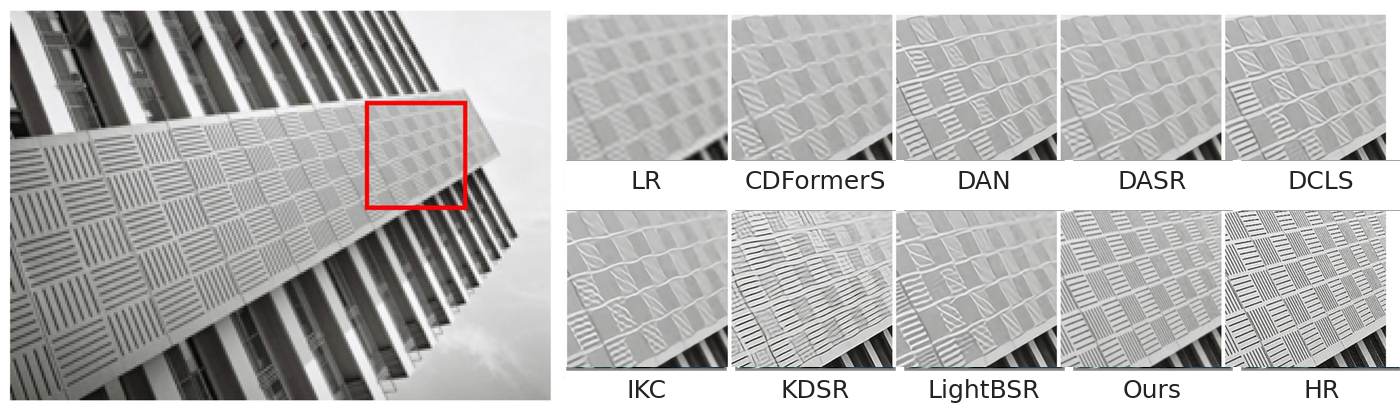
\includegraphics[width=.96\textwidth]{figures/img092_figure_font_matched.png}\\[4pt]
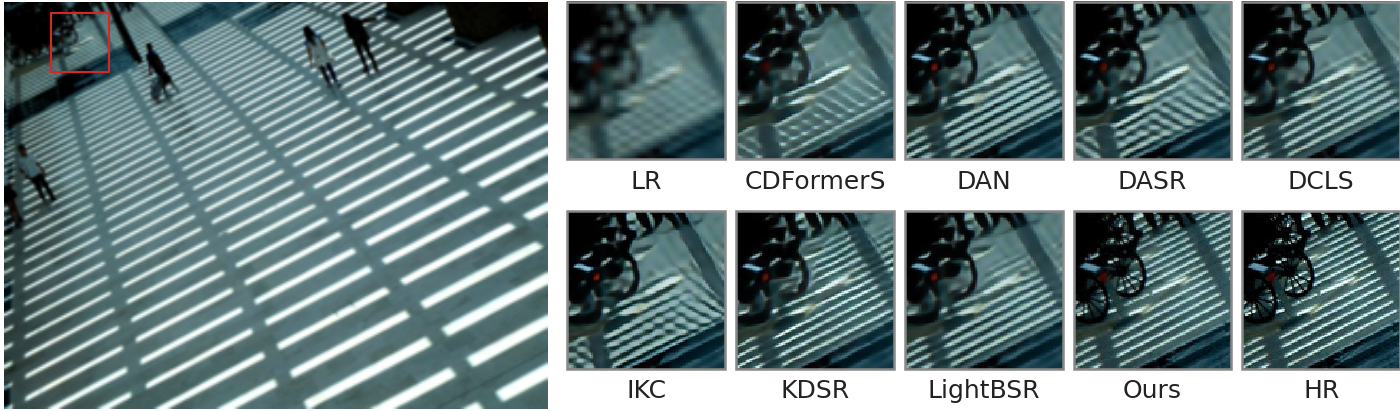
\includegraphics[width=.96\textwidth]{figures/img093_crops_grid_048style.png}
\caption{Qualitative comparisons on Urban100. The upper row shows the img092 building texture and the lower row shows the img093 crosswalk texture. Red boxes in the lower row indicate enlarged regions; each row includes the reconstructed crops and the HR reference.}
\label{fig:qualitative}
\end{figure*}

\subsection{Anisotropic Blur and Noise}
The anisotropic/noisy experiment extends the evaluation beyond noise-free isotropic degradation. Table~\ref{tab:anisotropic} compares DEDBSR with eight reference methods on B100 under the nine kernels and two noise levels of LightBSR Setting~2~\cite{yuan2025lightbsr}. Using the same architecture trained separately for this setting, DEDBSR achieves the highest or tied-highest PSNR in seventeen of the eighteen conditions. Relative to LightBSR, the mean improvements are 0.018 and 0.016~dB at noise levels 5 and 10; one condition is lower by 0.01~dB. Baseline scores follow the published comparison, and the full training degradation protocol is given in the supplement. Together with the isotropic results, this evaluation supports the architecture's applicability across distinct degradation settings. We next examine the condition path, residual composition, and LR-only adaptation directly.

% Full original method set. LightBSR corrected against official ICCV2025 Table 4.
% DEDBSR and all other baseline PSNR entries preserved from the archived full table.
\begin{table*}[!t]
\caption{B100 PSNR (dB) under nine anisotropic blur kernels and two noise levels for $\times4$ SR. Headers visualize the kernels in the order of LightBSR Table~4~\cite{yuan2025lightbsr}, which supplies the baseline scores. DEDBSR uses a separately trained anisotropic/noisy model. Bold/underline denote the best/second-best distinct scores, including ties.}
\label{tab:anisotropic}
\centering\footnotesize
\setlength{\tabcolsep}{4.5pt}
\renewcommand{\arraystretch}{1.03}
\begin{tabular}{clrrrrrrrrr}
\toprule
Noise & Method & \raisebox{-0.35\height}{
\includegraphics[height=0.25in]{figures/kernels/kernel_K1.png}} & \raisebox{-0.35\height}{
\includegraphics[height=0.25in]{figures/kernels/kernel_K2.png}} & \raisebox{-0.35\height}{
\includegraphics[height=0.25in]{figures/kernels/kernel_K3.png}} & \raisebox{-0.35\height}{
\includegraphics[height=0.25in]{figures/kernels/kernel_K4.png}} & \raisebox{-0.35\height}{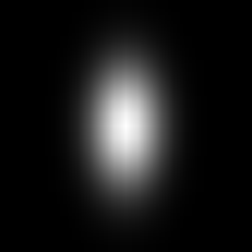
\includegraphics[height=0.25in]{figures/kernels/kernel_K5.png}} & \raisebox{-0.35\height}{
\includegraphics[height=0.25in]{figures/kernels/kernel_K6.png}} & \raisebox{-0.35\height}{
\includegraphics[height=0.25in]{figures/kernels/kernel_K7.png}} & \raisebox{-0.35\height}{
\includegraphics[height=0.25in]{figures/kernels/kernel_K8.png}} & \raisebox{-0.35\height}{
\includegraphics[height=0.25in]{figures/kernels/kernel_K9.png}}\\
\midrule
\multirow{9}{*}{5} & DnCNN+DAN & 26.18 & 26.14 & 24.89 & 24.64 & 24.61 & 24.52 & 24.37 & 24.01 & 23.63\\
 & DnCNN+DCLS & 26.15 & 26.12 & 24.89 & 24.66 & 24.62 & 24.52 & 24.39 & 24.03 & 23.65\\
 & DASR & 26.60 & 26.52 & 25.87 & 25.69 & 25.64 & 25.60 & 25.48 & 25.23 & 24.85\\
 & MRDA & 26.73 & 26.68 & 25.98 & 25.80 & 25.77 & 25.71 & 25.59 & 25.29 & 24.82\\
 & KDSR & 26.73 & 26.70 & 26.02 & 25.87 & 25.83 & 25.76 & 25.65 & 25.37 & 24.94\\
 & DSAT & 26.71 & 26.66 & 25.95 & 25.80 & 25.74 & 25.66 & 25.55 & 25.30 & 24.85\\
 & CDFormer-S & 26.77 & 26.69 & 26.00 & 25.85 & 25.82 & 25.75 & 25.64 & 25.34 & \second{24.97}\\
 & LightBSR & \second{26.82} & \second{26.76} & \second{26.06} & \second{25.91} & \second{25.87} & \second{25.81} & \second{25.70} & \best{25.41} & \best{25.05}\\
 & \textbf{DEDBSR} & \best{26.86} & \best{26.79} & \best{26.08} & \best{25.92} & \best{25.89} & \best{25.84} & \best{25.72} & \second{25.40} & \best{25.05}\\
\midrule
\multirow{9}{*}{10} & DnCNN+DAN & 25.69 & 25.63 & 24.62 & 24.42 & 24.39 & 24.29 & 24.18 & 23.89 & 23.54\\
 & DnCNN+DCLS & 25.67 & 25.62 & 24.62 & 24.43 & 24.40 & 24.29 & 24.19 & 23.91 & 23.56\\
 & DASR & 26.02 & 25.94 & 25.27 & 25.11 & 25.08 & 25.03 & 24.93 & 24.69 & 24.33\\
 & MRDA & 26.12 & 26.05 & 25.36 & 25.20 & 25.18 & 25.12 & 25.01 & 24.76 & 24.36\\
 & KDSR & 26.11 & 26.05 & 25.38 & 25.24 & 25.21 & 25.15 & 25.05 & 24.81 & \second{24.46}\\
 & DSAT & 26.07 & 26.04 & 25.29 & 25.18 & 25.14 & 25.09 & 24.97 & 24.72 & 24.36\\
 & CDFormer-S & 26.14 & 26.06 & 25.37 & 25.22 & 25.20 & 25.15 & 25.04 & 24.78 & 24.45\\
 & LightBSR & \second{26.18} & \second{26.10} & \second{25.41} & \second{25.27} & \second{25.24} & \second{25.19} & \second{25.08} & \second{24.83} & \best{24.53}\\
 & \textbf{DEDBSR} & \best{26.21} & \best{26.13} & \best{25.43} & \best{25.28} & \best{25.26} & \best{25.20} & \best{25.09} & \best{24.84} & \best{24.53}\\
\bottomrule
\end{tabular}
\end{table*}


\section{Ablation Studies and Analysis}
\subsection{Recurrent Condition Guidance}
We first examine how trained privileged branches depend on their condition paths, then test whether that dependence persists after recovery training. \emph{Nonrecurrent} retains group-specific update modules but computes each group's state from the initial conditions, preserving parameter count. \emph{One-shot} bypasses updates, and \emph{shared update} reuses the first group's update modules while retaining recurrence. The trunk, residual router, fusion, and output head remain fixed during the initial interventions; recovery training subsequently optimizes each variant's active modules.

Fixed-model interventions on two independently trained standard recurrent privileged branches reduce PSNR when recurrence is removed, bypassed, or shared. Removing recurrence loses 3.354--5.136~dB for the first branch and 4.113--5.255~dB for the second at the primary widths. Additional in-support widths show the same mean ordering, including a branch trained with an alternative update budget. The supplement reports the repeated-checkpoint and expanded-width tables, their paired intervals, and out-of-support exceptions. These interventions diagnose dependence on a trained condition path; matched recovery below tests whether its advantage persists after adaptation.

\noindent\textbf{Recovery after changing the condition path.}
Full retains the highest mean PSNR after matched recovery (Table~\ref{tab:shared_recovery}). All variants start from the same privileged checkpoint and receive equal recovery budgets. Full exceeds nonrecurrent, one-shot, and shared-update paths by 0.237, 0.250, and 0.026~dB, respectively. Against the equal-parameter nonrecurrent control, its paired image-bootstrap 95\% interval is $[0.182,0.302]$~dB; the Urban100 improvement is 0.524~dB. Recovery reduces the immediate intervention penalty but preserves a mean advantage for recurrent propagation.

\begin{table}[!t]
\caption{Matched recovery from the same teacher checkpoint: 30 epochs and 90,540 updates per variant. Mean averages twelve conditions; U100 averages three widths. Full and Nonrecurrent have equal active parameter counts. Complete dataset scores are in the supplement.}
\label{tab:shared_recovery}
\centering\scriptsize
\setlength{\tabcolsep}{3pt}
\begin{tabular}{lrrr}
\toprule
Condition path & Mean PSNR & U100 PSNR & Mean SSIM\\
\midrule
Full & 28.466 & 25.843 & .79322\\
Nonrecurrent & 28.230 & 25.319 & .79133\\
One-shot & 28.216 & 25.299 & .79103\\
Shared update & 28.440 & 25.785 & .79304\\
\bottomrule
\end{tabular}
\end{table}


\subsection{Depth and Residual Composition}
\label{sec:depth}

\noindent\textbf{Depth-dependent restoration.}
The reported architectural sweep in Fig.~\ref{fig:motivation}(a) reaches its highest twelve-condition mean at ten blocks per group, which we retain as the benchmark reference configuration. The separate depth retest uses different training conditions; the supplement records the provenance and protocol limitations of these comparisons.

Our Fourier analysis examines the reconstruction obtained by executing different numbers of blocks within every group of a trained network. On 100 Urban100 images at three blur widths, the full execution prefix has lower mean normalized complex HR error than the shortest prefix in all nine blur--frequency conditions. The final output increment also aligns with the missing HR residual. These observations show that additional computation within the probed networks can contribute useful reconstruction corrections, motivating the transfer of a restoration path that retains this computation. The trained condition updates, group tails, and reconstruction head remain active throughout the probe; the complete protocol is given in the supplement.


\noindent\textbf{Degradation-guided stage composition.}
The composition probe retains all completed group corrections and varies how they are combined. Extending Fig.~\ref{fig:motivation}(b), combination prototypes are estimated on one image split and evaluated on a held-out split across seven blur widths. Matched combinations exceed alternatives by 0.530~dB on Urban100 and 0.410~dB on B100 on average, showing that reconstruction depends on stage composition. The matched uniform-weight retraining control reaches similar mean PSNR (differences below 0.006~dB; supplement), so these observations establish composition sensitivity without establishing an independent accuracy gain from input-dependent weighting.

\begin{figure}[!t]
\centering
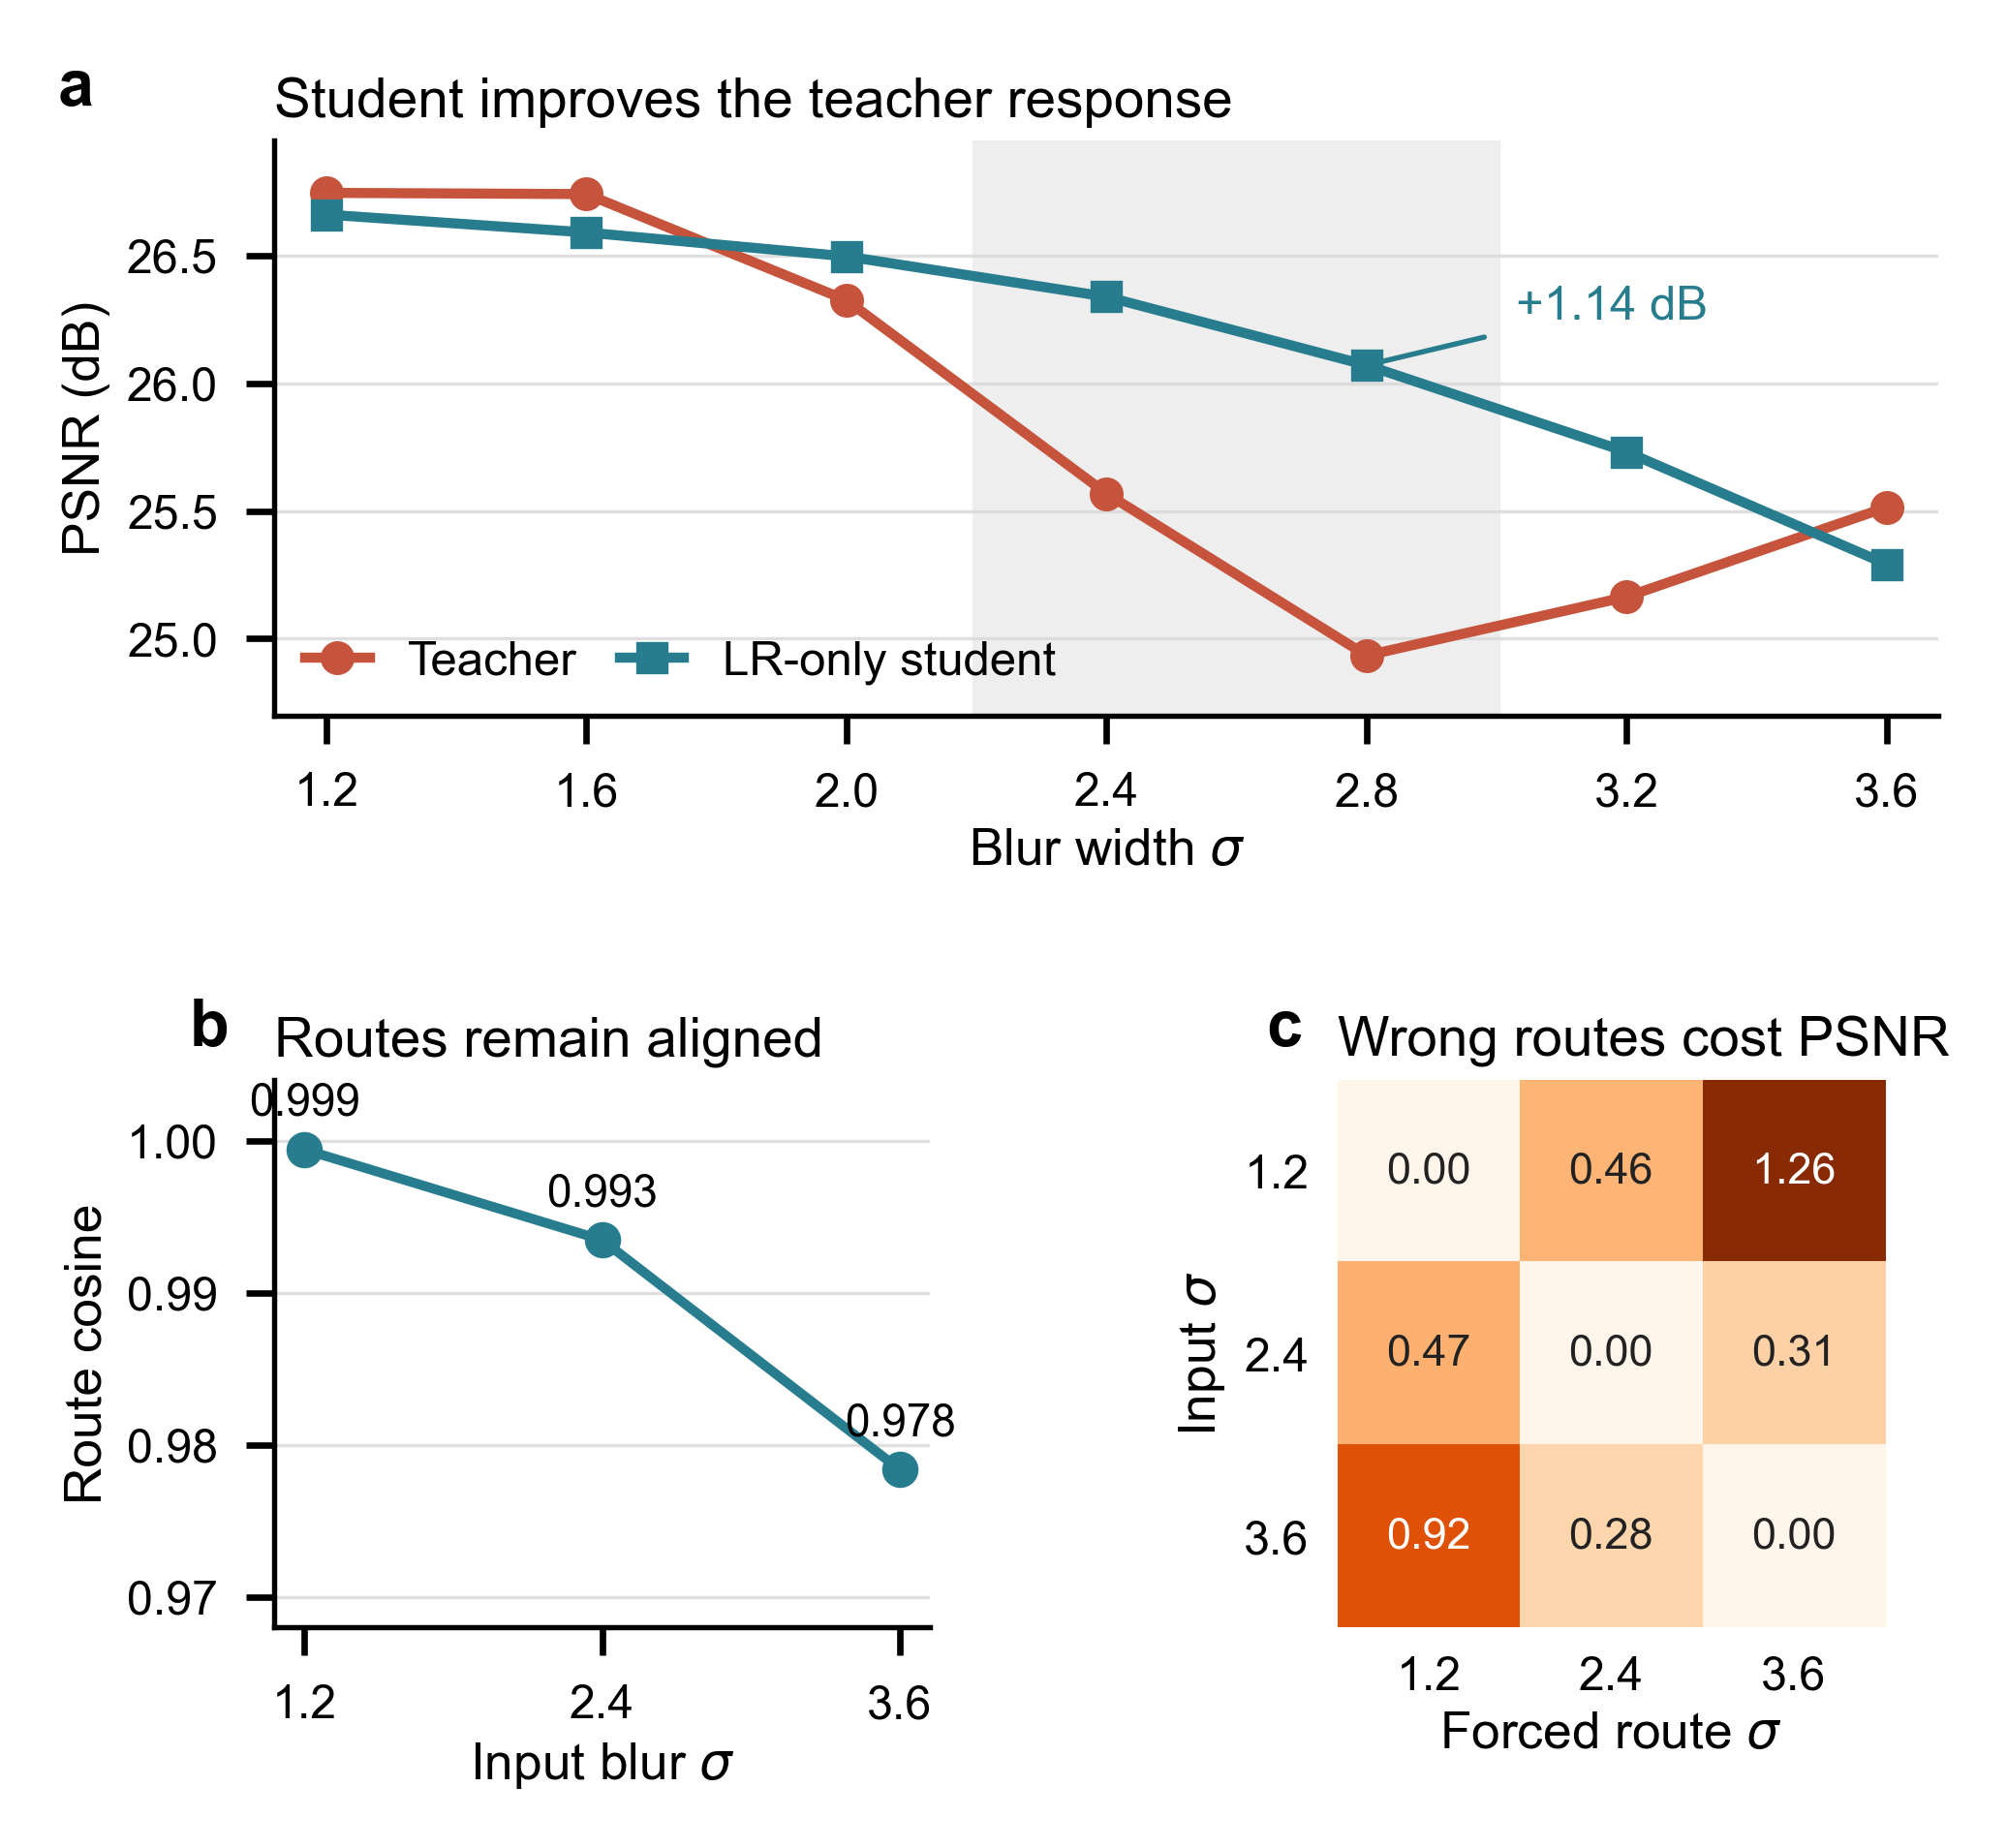
\includegraphics[width=\columnwidth]{figures/fig_transfer_interface_main.png}
\caption{\textbf{Distillation and LR-only adaptation diagnostics.} (a) PSNR of the privileged and LR-only branches across blur widths; (b) cosine similarity of their residual routes; (c) PSNR loss after forcing a route from another blur width. The probe quantifies LR-only adaptation and route consistency; complete gate diagnostics are provided in the supplement.}
\label{fig:transfer}
\end{figure}

\subsection{Initialization and LR-only Adaptation}
\begin{table}[!t]
\caption{Initialization and adaptation at the selected student checkpoint. Mean/U100 average twelve/three conditions. The GT-only rows compare initialization; Full versus F5 tests adaptation. Schedules and full objectives are in the supplement.}
\label{tab:controls}
\centering\scriptsize
\setlength{\tabcolsep}{2.1pt}
\renewcommand{\arraystretch}{1.06}
\resizebox{\columnwidth}{!}{%
\begin{tabular}{lrrrr}
\toprule
Configuration & Mean PSNR & U100 PSNR & Mean SSIM & U100 SSIM\\
\midrule
\multicolumn{5}{l}{\textit{Initialization under GT-only reconstruction}}\\
GT-only, scratch & 28.430 & 25.940 & -- & --\\
GT-only, initialized & 28.504 & 26.129 & .7905 & .7809\\
\midrule
\multicolumn{5}{l}{\textit{Adapting the inherited restoration network}}\\
Full & 28.513 & 26.108 & .7903 & .7796\\
F5: frozen restoration & 28.257 & 25.585 & .7851 & .7654\\
\bottomrule
\end{tabular}
}%

\end{table}



\noindent\textbf{Initialization and adaptation.}
The initialization and adaptation controls isolate the effect of transferring a trained restoration structure. Under GT-only reconstruction, privileged initialization raises mean PSNR from 28.430 to 28.504~dB and the Urban100 mean from 25.940 to 26.129~dB. Freezing the inherited restoration network reduces Full by 0.256~dB overall and 0.523~dB on Urban100. These controls support transferring a trained restoration structure and subsequently adapting it to LR-derived conditions.



\noindent\textbf{GT-referenced output selection.}
Figure~\ref{fig:transfer} shows that the LR-only branch can adapt beyond weaker privileged predictions while retaining similar residual routes, with PSNR improvements of up to 1.14~dB in the interior blur interval. In the fixed-patch probe, direct output imitation is disabled on all 138 privileged-worse patches while GT reconstruction remains active, verifying the intended selection rule. In matched three-epoch recovery, Gate-on, Gate-off, and No-output-KD reach 28.5203, 28.5280, and 28.5170~dB, respectively. These finite-budget controls do not establish an independent accuracy gain from the gate; complete protocols and fixed-patch results are provided in the supplement.

\section{Conclusion and Discussion}
DEDBSR transfers a condition-guided restoration path from a kernel-informed privileged branch to an LR-only branch. Recurrent channel and spatial states guide successive groups, and a degradation-guided ensemble combines their corrections. GT provides reconstruction targets and selects output imitation. Across the reported protocols, DEDBSR achieves leading PSNR in most evaluated conditions. Initialization and adaptation controls support transferring trained restoration computation, while matched recovery supports recurrent propagation within the measured training range.

The framework couples inherited restoration computation with GT-referenced target selection. The LR-only branch inherits and adapts the restoration path, with GT reconstruction active for every adaptation sample and output imitation selected by relative error. Extending this approach to broader real-world degradations is a direction for future work.

\begingroup
\emergencystretch=2em
\tolerance=2000
\bibliographystyle{IEEEtran}
\bibliography{references}
\endgroup
\end{document}









